%%=============================================================================
%% Eventual Consistency
%%=============================================================================

\section{Eventual Consistency}
\label{sec:eventual-consistency}

Elk commando dat in het systeem terecht komt, kan op een queue geplaatst worden. Het grote voordeel hier van is dat het systeem niet over belast wordt en dat elke queue job afgehandeld kan worden \autocite{King2015EventualConsistency}. Vandaar de term eventual consistency, uiteindelijk zal het systeem consistent zijn. Een ander groot voordeel is dat eventual consistency automatisch samen kan werken met schaalbaarheid van een applicatie, zoals beschreven in Hoofdstuk~\ref{ch:schaalbaarheid}. Wanneer er een commando uitgevoerd wordt op het systeem, weet de client al de data al. Er is momenteel geen nood om meteen een response terug te krijgen.
Daarom is het ook belangrijk bij commands om een \gls{GUID} op voorhand te definiëren zodat de identiteit al bekend is. Met deze identiteit kan er eventueel al een pagina getoond worden waar de data getoond wordt.

\begin{figure}[h]
\caption{Eventual Consistency}
\centering
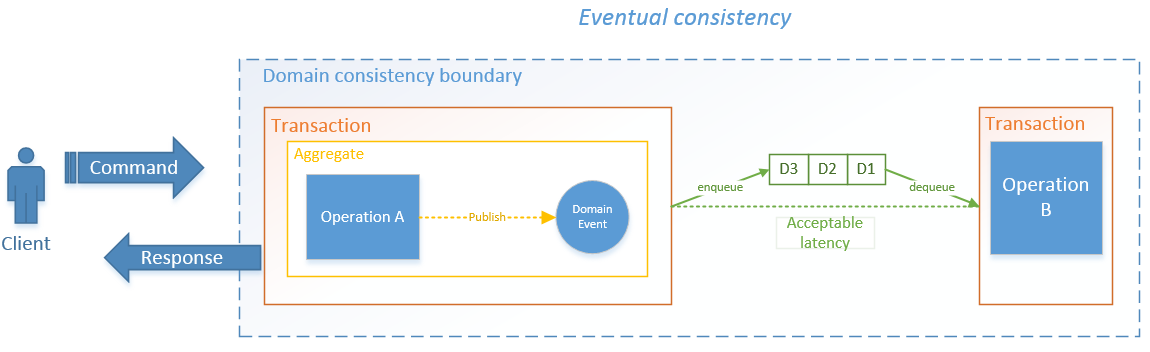
\includegraphics[width=0.75\textwidth]{img/eventual-consistency}
\end{figure}

\subsection{Transactional Consistency}
\label{subsec:transactional-consistency}

Het voordeel aan transactional consistency is dat de response meteen terug gegeven wordt. Alle delen van de applicatie zijn doorlopen en alle gegevens zijn gepersisteerd. Het grote nadeel is dat de applicatie volledig doorlopen moet worden en dat de response veel trager kan zijn. Indien de applicatie exponentieel hoog aantal requests binnen krijgt en dus alles meteen moet afhandelen. Kan dit resulteren in het crashen van de applicatie.
Transactional consistency is ook moeilijker schaalbaar omdat alles in 1 keer uitgevoerd wordt.

\begin{figure}[h]
\caption{Transactional Consistency}
\centering
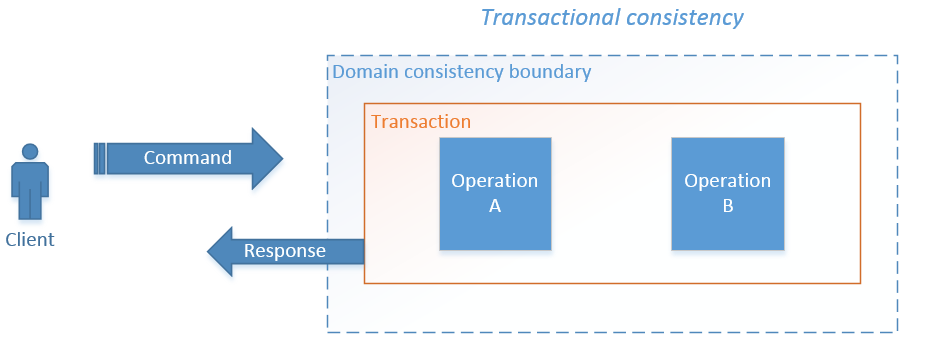
\includegraphics[width=0.75\textwidth]{img/transactional-consistency}
\end{figure}
